\section{Component Densities}

\begin{figure}[h!]
\begin{center}
	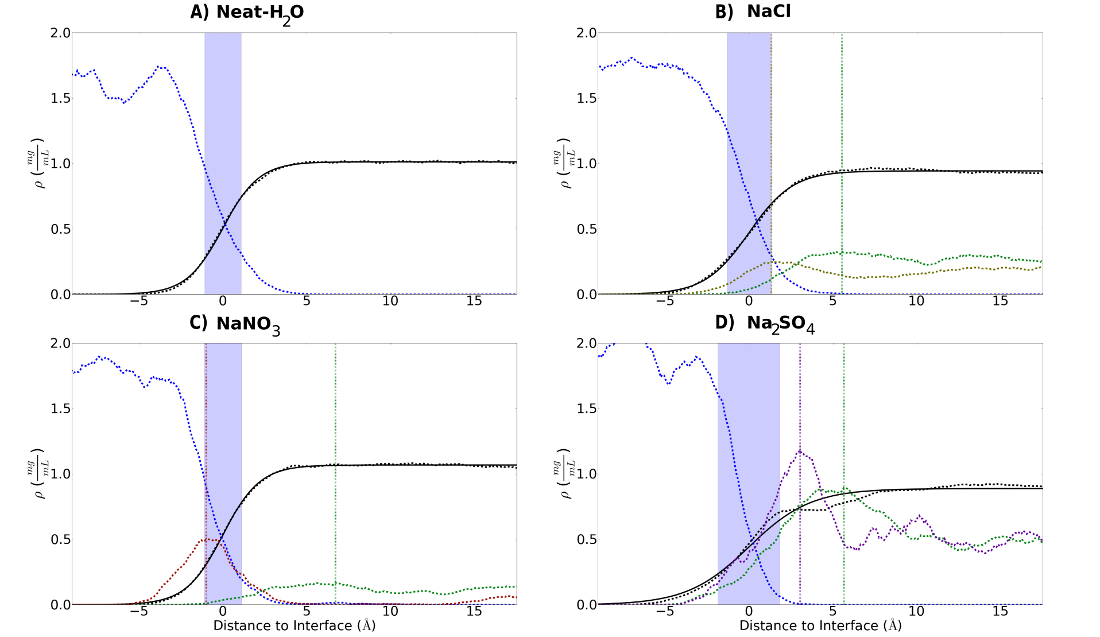
\includegraphics[scale=1.0]{images/densities.png}
	\caption{Aqueous salt solution (1.2 M) and CCl$_4$ surface density profiles. (A) Neat-H$_2$O, (B) NaCl, (C) NaNO$_3$, and (D) Na$_2$SO$_4$ aqueous solution densities are plotted with the water-oxygen density (dashed black) and the corresponding fitted lineshape (solid black). The CCl$_4$ (dashed blue), Na$^+$ cation (dashed green, scaled 10x) and respective anion (scaled 5x) densities are also shown for each system. The maxima of the ionic components are marked with dashed vertical lines of the same colors.}
	\label{fig:density-plots}
\end{center}
\end{figure}

The component density profiles of each system were calculated to study the effects of added salts on water's density profile, and to find any deviations from the \ctcwat system. The water density profile of each system was fitted to a hyperbolic tangent function (Eq. \ref{tanh_fit}). The resulting plots are shown in figure \ref{fig:density-plots}. The profiles were centered about the GDS locations, $z_0$, at 0.0\angs, and all lineshapes are plotted as distances to the GDS. Each interfacial width, $d$, is designated as a highlighted blue region of width $d$ centered about $z_0$.  The widths of the interfacial regions for the neat-H$_2$O (A), NaCl (B), NaNO$_3$ (C), and Na$_2$SO$_4$ (D) systems are 2.16, 2.62, 2.20, 3.69\angs, respectively. In each of the salt solutions, the anion density profile shows enhancement near the interface, appearing as a peak in the profile. These anion enhancements all occur closer to the interface than the corresponding counter-cation. Various parameters of interest such as the interfacial thicknesses, ionic enhancement locations (taken to be the location of the maxima in the ion profiles near the interface), and relative distances between the peaks of the ion profiles are collected in table \ref{table:double-layer}.

\begin{table}[htdp]
	\begin{center}
	\begin{tabular}{|c||c|c|c|c|}
		\hline
		System & $d$ & Anion & Cation & Anion-Cation Distance \\ \hline
		Neat-H$_2$O & 2.16 & - & - & - \\ 
		NaCl & 2.62 & 1.33 & 5.53 & 4.20 \\
		NaNO$_3$ & 2.20 & -0.99 & 6.71 & 7.70 \\
		Na$_2$SO$_4$ & 3.69 & 3.04 & 5.64 & 2.60 \\
		\hline
	\end{tabular}
	\end{center}
	\caption{Aqueous salt system density parameters. Interfacial widths, $d$, and the locations of the maxima of the density profiles for each ionic component are listed for the simulated salt systems. The relative distances between the anion and cation density peak locations are listed to show how the different anions affect the relative location of their cationic counter-ions.}
	\label{table:double-layer}
\end{table}

The oscillations in the surface density profiles of water and the adjoining organic \ctc liquid phase have been noted previously and attributed to thermal capillary waves on a larger length-scale than the simulated system size.\cite{Chang1996} The same work also made note that the interfacial thickness is size-dependent on the interfacial surface area. Increasing the surface area dimensions should therefor cause an increase in the interfacial width. As a consequence, care must be taken when making quantitative comparisons between widths and locations found in differing simulation studies. Two works on the \ctcwat surface offer direct comparison of this.\cite{Chang1996,Hore2008}

In comparing the three salt solutions studied here, any differences in those systems are anionic in nature because the cation of each system was kept the same. \nacl is the simplest of the three salts with a monatomic and monovalent anion. The peak of the anion density profile is within the aqueous phase (i.e. it is found on the aqueous-side of the interfacial width). The location of the cation density peak is, as mentioned above, deeper into the aqueous phase than the anion by over 4\angs. This layering of ions within the aqueous phase is attributed to the break in the anisotropy of the field of the bulk region upon introduction of the organic phase. The more polarizable and negatively charged anions move towards the interface to effectively screen the induced field from the organic phase and the more highly ordered water structure near to it. The counter-ions then are drawn towards the negative charge built up by the anions to create the second ion density peak deeper into the aqueous phase. The overall shape of the water profile in the \nacl system is relatively unaffected (compared to the neat-\wat) by the presence of the ions. The bulk water density is unchanged, and the width of the interface is only slightly increased above that of neat-\wat.

In an MD study of \ctcwat interfaces by Wick and Dang,\cite{Wick2007a} larger and more polarizable monovalent anions were found to be less solvated and exhibited a smaller density enhancement when compared to the \airwat interface. The \ctcwat interface was found to be a less favorable solvation environment for the more polarizable anions. A break in the isotropic environment around the ions causes them to be less solvated and come in greater contact with the \ctc phase. The ions are thus pushed further into the aqueous bulk than at an air-interface. However, the surface activities and density enhancements of the more polarizable anions (i.e. I$^-$, Br$^-$) remain greater than that of a smaller and less polarizable one (i.e. Cl$^-$) at both interfaces. 
%Few surface-specific experimental analyses (i.e. SFG) have been performed on these \ctc systems and were mostly limited to the \airwat surface.

With respect to the surface waters, strengthening of the interfacial hydrogen-bonding structure may allow them to further penetrate into a second, organic phase, thus widening the interface region and enhance SFG intensity from interfacial hydrogen-bonded species. We find this to be true when comparing interfacial widths from our simulations. Those ions that are best known to enhance the strength of hydrogen-bonding produce wider interfaces with greater water penetration into the \ctc phase.

The \sodnit system introduces the monovalent, polyatomic nitrate anion. The location preference of nitrate is a contentious subject that has been studied much in recent years at the air-\wat interface,\cite{Brown2009,Thomas2007} but very little at an organic-\wat interface. We find a strong surface enhancement of the nitrate anion like other monovalent ions that have been analyzed in the \ctcwat environment.\cite{Wick2007a} The nitrate density peak is located the furthest out from the aqueous phase of the three salt systems, as expected by its high polarizability. The location of the sodium cation peak in this system is a significant distance further into the bulk from the anion than in either of the \nacl or \sodsul systems. The increase in ion-pair distance may be the result of strong screening of the interfacial field by the surface-active anion, and the solvating waters around it. The interfacial width of this system is the narrowest of our study. Water's ability to extend into the organic phase is affected by its hydrogen-bond network strength. Nitrate acting to break the surface water bonding thus decreases the width of the water penetration into the organic phase. 

%Such surface location and enhancement of the nitrate ion suggests a very strong interaction with the interface waters, breaking the hydrogen-bonding network near to the organic phase, and also strongly screening the field of the \ctc molecules from the interface. This accounts for the narrower interfacial width as the water can no longer extend a bonded network into the organic phase. As the water is strongly interacting with the nitrate and effectively screening the field from the surface, the counter-cation is less attracted to the interface and the ionic double-layer is widened. 

The widest interface is that of the \sodsul solution, indicating that the \sul anions act to strengthen greatly the hydrogen-bonding network between the surface waters. The location of the \sul density enhancement is the furthest into the aqueous bulk of the three anions, and the divalent and highly polarizable nature of the anion appears to attract the counter-ion closest for the narrowest sub-surface ionic double-layer. This attraction is likely coulombic, and the charge screening that separates the ion pairs in the \sodnit solution is not present in aqueous \sodsul. Although the greatest concentration enhancement is further into the bulk region, seemingly outside the region designated by the interfacial width, the water hydrogen-bonding network is still greatly enhanced. This has been verified by an increase in SFG response of the surface waters relative to the neat-water system in a recent experimental study by this group.\cite{McFearin2009}


%comparison to air-water
The neat-\airwat system is the acting benchmark and has been simulated and analyzed previously.\cite{Wick2006c,Hore2008,Wick2008a} Deviations in width of the interface from the neat-\ctcwat system can be attributed to the added ions in the solution. One work used SFG to detect structural changes in the water hydrogen-bonding network at the air interface in the presence of various anions, and found that it affects the SFG signal intensity from the interface, but could not create the anion density profile\cite{Schnitzer2000}. The same work found SFG intensity enhancement for hydrogen-bonded water following a trend of H$_2$SO$_4\ge$ HCl $>$ HNO$_3$. Comparison with an \airwat MD study complements this trend finding that the \sul concentration enhancement was found furthest into the water bulk.\cite{Salvador2003} Although the SFG studies stopped short of reporting a concentration profile, a recent X-ray photo-emission spectroscopy study was performed to specifically determine the nitrate concentration profile for the water-vapor interface, and reported the current differences of opinion between experiment and simulation.\cite{Brown2009} The XPS results showed a surface depletion of the nitrate anion relative to the bulk, similar to previous MD simulations of the same systems. Other works performed on the liquid-vapor interface found similar nitrate surface depletions.\cite{Otten2007} These help to contrast the effect of the presence of an organic phase as in the present work. 

Xu, et al, studied this phenomena finding a lack of ion-pairing of various nitrates at the \airwat interface.\cite{Xu2009} They found that solvation from an abundance of water at the interface weakens coulombic forces between ions, leading to greater cation-anion separation. They concluded that the surface nitrate is dehydrated, and the water provides adequate shielding of the ionic coulombic interactions. It is reasonable to assume that this same effect may cause the greater cation-anion separation at the interface of the \sodnit system, even in the presence of the organic phase.

Behavior of monovalent ions at the \ctcwat interface is clearly different than that of \airwat systems. Previous simulations found concentrations of small monovalent anions to be lower at the \ctcwat interface than at the air-liquid one.\cite{Wick2007a} Most of the recent studies on ion concentration near water interfaces have noted that large and polarizable ions will concentrate at the air surface,\cite{Petersen2005b,Pegram2006,Sloutskin2007,Eggimann2008} while small non-polarizable ions tend to be repelled. The surface enhancement calculated from those MD studies, however, portrays the lower bound of the actual effect because of the reduced polarizability values used in simulations to avoid the so-called ``polarization catastrophe.'' The enhancement of surface anions is also believed to be the cause of the subsurface cation density increase. The counter-ions are attracted to the concentrations of anions at the surface, which are in turn stabilized by the increased polarization of the water due to the distorted interfacial electric field. The affinity for the surface follows the trend of surface tension increments, $\frac{d\gamma}{dm_2}$, where Na$_2$SO$_4 >$ NaCl $>$ NaNO$_3$.\cite{Pegram2006} This also follows the Hoffmeister series trend for anions found to be the most ``structure-making'', and they are found to be density enhanced further into the interface. Our simulations for this work thus provide an interesting comparison to the \airwat research, and the analysis shows evidence that an organic phase causes changes in behavior of the surface waters.

%Ionic density profiles were fitted by adding a Gaussian function to the hyperbolic tangent function (Eq. \ref{ion_fit}) to more closely capture the concentration enhancement excess near or within the interfacial region. The lineshape parameters for each salt system are shown in table \ref{ion_params}.

%\begin{table}[htdp]
	%\begin{center}
	%%system; Anion: (a,b,c,Z0,d); Cation: (a,b,c,Z0,d)
	%\begin{tabular}{c|c|c|c|c|c|c|c|c|c|c|}
		%\cline{2-11}
		%\multicolumn{1}{c|}{} & \multicolumn{5}{c}{Anion} & \multicolumn{5}{|c|}{Cation} \\ 
		%\cline{1-11}
		%\multicolumn{1}{|c|}{System} & $a$ & $b$ & $c$ & $z_0$ & $d$ & $a$ & $b$ & $c$ & $z_0$ & $d$ \\ \hline
		%\multicolumn{1}{|c|}{NaCl} & 0.464 & -1.726 & 1.361 & -3.190 & 1.928 & -0.257 & -8.252 & 2.154 & -2.278 & 1.666 \\ \hline
		%\multicolumn{1}{|c|}{NaNO$_3$} & 0.732 & 0.655 & 1.520 & -0.962 & 0.407 & 0.335 & -1.614 & 1.982 & -2.769 & 1.384 \\ \hline
		%\multicolumn{1}{|c|}{Na$_2$SO$_4$} & 0.474 & -3.551 & 1.162 & -5.594 & 2.307 & -0.707 & -8.648 & 3.439 & -3.203 & 1.791 \\ \hline
	%\end{tabular}
	%\end{center}
	%\caption{Lineshape fitting parameters for the ion density profiles. The data for each density profile is fit to a convolution of a hyperbolic tangent and Gaussian peak functions (Eq. \ref{ion_fit}). The parameters $a$, $b$, and $c$ are used for fitting the Gaussian peak to model the concentration of ion near to the interfacial region. $z_0$ and $d$ are the two parameters used to model the hyperbolic tangent lineshape for the bulk concentration and the decrease of density within the H$_2$O-CCl$_4$ interface.}
	%\label{ion_params}
%\end{table}

